\documentclass[11pt,a4paper]{article}
\usepackage{fullpage}
\usepackage{tgadventor}
\usepackage[T1]{fontenc}
\newcommand{\hsp}{\hspace{20pt}}
\newcommand{\HRule}{\rule{\linewidth}{0.5mm}}
\usepackage{float}
\usepackage{amsmath}
\usepackage{caption}
\usepackage{subcaption}
\usepackage{graphicx}
\usepackage{xcolor}
\usepackage{multirow}
\usepackage{hyperref}
\definecolor{darkblue}{RGB}{14,43,88}
\usepackage{chemformula}

\makeatletter
\newcommand{\authors}{%
  \setlength\arrayrulewidth{2pt}
  \begin{tabular}{l|l}
  \@authorsi
}
\newcommand\@authorsi{\@ifnextchar\stopauthors{\@authorsend}{\@authorsii}}
\newcommand\@authorsii[2]{%
  \\
  \textbf{\Large #1} &  \textbf{\Large #2}
  \\
  \@authorsi % restart the recursion
}
\newcommand\@authorsend[1]{
  \end{tabular}}
\makeatother

%%%%%%%%%%%%%%%%%%%%%%%%%%%%%%%%%%%%%%%%%%%%%%%%%%%
%%%%%%%%%%%% Define following Variables %%%%%%%%%%%
%%%%%%%%%%%%%%%%%%%%%%%%%%%%%%%%%%%%%%%%%%%%%%%%%%%
\def \classSigle{LMAPR2451}
\def \className{Atomistic and nanoscopic simulations}
\def \workName{Study of \ch{FeS2} and its optical properties}
\def \professors{Professors Jean-Christophe Charlier, Xavier Gonze \& Gian-Marco Rignanese\\Mentors : Alexandre Cloots \& Ionel-Bogdan Guster}
\def \academicYear{2020-2021}
\def \abstractText{This report aims to investigate the optical properties of \ch{FeS2}. To do so, \textit{ab initio} computations are performed on a 6-atoms orthorhombic unit cell. The convergence with respect to several structural parameters is also studied. The optical properties are then analyzed in the light of the obtained results. Finally, a comparison is made with the published research, and a discussion about the quality of the simulation is made.}
%%%%%%%%%%%%%%%%%%%%%%%%%%%%%%%%%%%%%%%%%%%%%%%%%%%
%%%%%%%%%%%%%%%%%%%%%%%%%%%%%%%%%%%%%%%%%%%%%%%%%%%
%%%%%%%%%%%%%%%%%%%%%%%%%%%%%%%%%%%%%%%%%%%%%%%%%%%

\begin{document}
\begin{titlepage}
\begingroup
\fontfamily{\sfdefault}
  \begin{flushleft}  
  \begin{minipage}{0.55\textwidth}  
\includegraphics[width=\textwidth]{images/epl2.png}
  \end{minipage}
  \end{flushleft}
  \centering
  \textcolor{darkblue}{{\huge \textbf{\classSigle \\[0.1cm] \className}}}
  \vfill
  \textcolor{darkblue}{
  \hrule height 0.1cm
  \hspace{1cm}\\[0.3cm]
  {\Huge \textbf{\workName}}\\[0.5cm]
  \hrule height 0.1cm
  \hspace{1cm}\\[0.3cm]
  {\Large\textbf{\professors}}}
  \vfill
  \begin{minipage}[c]{\textwidth}
  \centering
  \textcolor{darkblue}{
  \authors
  %%%%%%%%%%%%%%%%%%%%%%%%%%%%%%%%%%%%%%%%%%%%%%%%%
  %%%%Mettre un auteur par ligne sous le format%%%%
  %%%%%%%%%%%%%%%%{Nom Prénom}{NOMA}%%%%%%%%%%%%%%%
  %%%%%%%%%%%%%%%%%%%%%%%%%%%%%%%%%%%%%%%%%%%%%%%%%
  {Anatole Moureaux}{54731700}
  %%%%%%%%%%%%%%%%%%%%%%%%%%%%%%%%%%%%%%%%%%%%%%%%%
  %%%%%%%%%%%%%%%%%%%%%%%%%%%%%%%%%%%%%%%%%%%%%%%%%
  %%%%%%%%%%%%%%%%%%%%%%%%%%%%%%%%%%%%%%%%%%%%%%%%%
  \stopauthors}
  \end{minipage}
  \vfill
  \noindent\fbox{%
    \parbox{1\textwidth}{%
        \centering
         \textcolor{darkblue}{\textbf{\abstractText}}%
        }
    }
  \vfill
  \begin{center}
  \textcolor{darkblue}{\textbf{\Large \academicYear}}
  \end{center}
\endgroup
\end{titlepage}
\tableofcontents
\newpage
\section{Introduction}
\subsection{Motivation}
Pyrite (\ch{FeS2}) is an interesting semiconducting material. Indeed, it can be used in numerous domains, from mechanical applications, where it is appreciated for its toughness and abrasiveness, to optical applications, where it can be used as an high-energy light absorber \cite{pyriteApps}. As pyrite is very abundant, it can become a material of choice in the industry if correct and valuable uses of the latter could be elaborated. It is depicted on \autoref{fig:pyriteOre}.

\begin{figure}[H]
\centering
\begin{subfigure}[b]{0.45\textwidth}
\centering
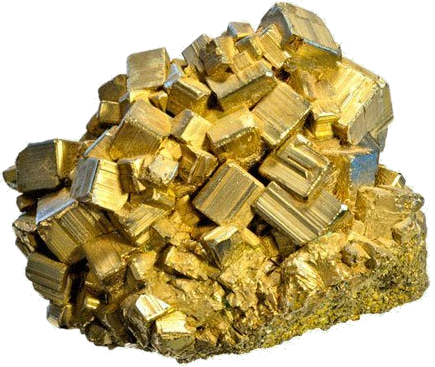
\includegraphics[width=\textwidth]{images/pyrite}
\caption{Pyrite}
\label{fig:pyriteOre}
\end{subfigure}
\hfill
\begin{subfigure}[b]{0.45\textwidth}
\centering
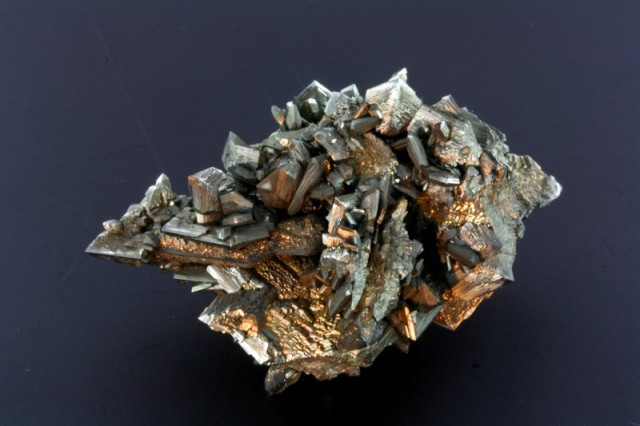
\includegraphics[width=\textwidth]{images/marcassite}
\caption{Marcassite, the orthrhombic polymorph of pyrite}
\label{fig:marcassiteOre}
\end{subfigure}
\caption{\ch{FeS2} ores}
\end{figure}

One of the promising potential application of pyrite is its integration into solar panels. Indeed, pyrite thin films could be good alternatives to the conventional silicon based solar cells, since the latter are more economically and ecologically costly \cite{pyriteSolarCells,Ore}. However, the performances of the material must be similar to or better than materials already used for solar cells, in order to make it truly competitive.

The concept of solar cell dates all the way back to 1883 \cite{solarcellinvention}. However, it is interesting to recall some of the main features of such a device. A solar cell consists of photoelectric components able to convert the energy of the (solar) light into electricity though the \textit{photovoltaic effect}. More precisely, it is composed of a \textit{pn}-junction diode, usually made of silicon. When the depletion region of the junction is hit by solar photons, an electron is delivered in the $n$-layer and a hole is delivered in the $p$-layer (\autoref{fig:pnjunction}). By doing so on a large scale, the \textit{pn}-junction is able to generate a voltage of about $0.5$ V, if the $n$-doped layer is sufficiently thin (to make the photons reach the depletion region as easily as possible). A solar panel is composed of several solar cells in series, in order to add up the voltage generated by each cell. The best materials for solar cells-related applications are the materials showing :
\begin{itemize}
\item a semiconducting behavior
\item a high optical absorption coefficient
\item a high electrical conductivity
\item an abundant presence in the Earth's crust.\cite{solarCell}
\end{itemize}
\begin{figure}[H]
\centering
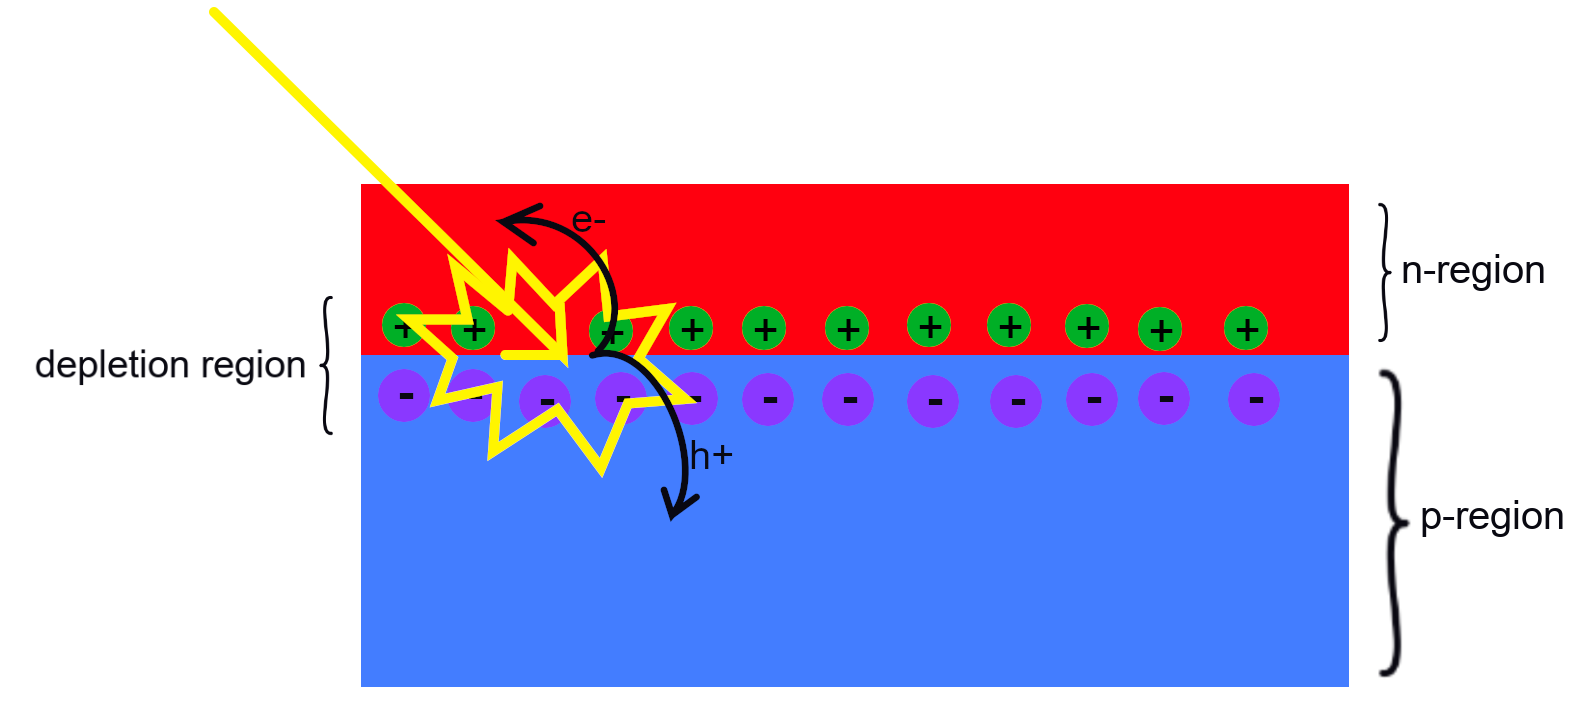
\includegraphics[width=0.8\textwidth]{images/pnjunction.png}
\caption{Simplified view of the photovoltaic effect at the $pn$-junction of a solar cell. The green and purple dots are the charges resulting from the recombination of charge carriers in the depletion region. When a photon hits an atom in the depletion region, an electron is released in the $n$-region and a hole is released in the $p$-region, creating a voltage when repeated multiple times.}
\label{fig:pnjunction}
\end{figure}
Even if bulk pyrite shows a $n$-type behavior, pyrite thin-films show a $p$-type behavior. Only the deposition of a thin layer of $n$-type semiconductor on the pyrite film is needed to form a $pn$-heterojunction. Furthermore, the pyrite has a strong absorption coefficient. It thus allows to decrease the thickness of the pyrite film, which is helpful to improve the performances of the $pn$-junction, and hence, of the solar cell \cite{thinFilms}. Furthermore, it is earth-abundant. Pyrite thus seems to be a material of choice for photovoltaic applications.

However, serious limitations prevent pyrite to be highly performant in this framework. Indeed, a very poor solar energy conversion efficiency is observed when assessing the performances of pyrite solar cells. That low efficiency is presumably due to a low photovoltage generation. The origin of that low photovoltage is highly debated among the scientific community. Several possible sources have been proposed over the years : detrimental \ch{S} vacancies (although stoichimetric pyrite shows the same low photovoltage), detrimental impurities or even lattice defects \cite{limitations}. No consensus has been found so far. But as pyrite could be a game-changer in the solar cell industry if its efficiency were improved, it is worth to look a little closer to the optical properties of the material.

In the following report, the properties of the \ch{FeS2} in the Pnnm space group will be studied using the \texttt{Abinit} package \cite{Abinit}. As the unit cell of pyrite, which contains 12 atoms, is close to the computational limits of \texttt{Abinit}, the computations will be performed on a 6-atoms orthorhombic polymorph, depicted on \autoref{fig:marcassiteOre}. The results will be used as a starting point for the reflection concerning the actual pyrite. First, the unit cell and its structural parameters will be described, based on the Materials Project documentation\footnote{\url{https://materialsproject.org/materials/mp-1522/}}. Then, the representation of the crystal in \texttt{Abinit} will be presented. Secondly, the pseudopotential and the approximation used in the first place will be discussed. Then, the convergence of the total energy per atom and the lattice scale parameters, with respect to the energy cut-off (\texttt{ecut}) and the number of $k$-points (\texttt{ngkpt}) will be studied. After that, \texttt{Abinit} computations will be performed using the converged values and the optical properties will be studied. To conclude, the obtained results will be compared with the published research.
\subsection{\ch{FeS2} : Overview and \texttt{Abinit} representation}
The orthorhombic \ch{FeS2} primitive cell contains 2 Fe atoms and 4 S atoms (\autoref{fig:primitiveCell}). The space group is Pnnm[58] in the Hermann-Mauguin notation. 

Furthermore, it is a semiconductor. The energy of the indirect bandgap is about 0.978 eV\cite{MaterialsProject}.

Finally, the primitive cell will be represented as follow in \texttt{Abinit} input files :
\begin{center}
\begin{tabular}{lll}
\texttt{acell} & \texttt{3.390} \texttt{4.438} \texttt{5.411} \texttt{Angstr} & \texttt{\# the lattice vectors scaling}\\
\texttt{ntypat} & \texttt{2} & \texttt{\# there are two types of atoms in the}\\
&&\texttt{\#\space\space\space\space primitive cell : Fe and S}\\
\texttt{znucl} & \texttt{26 16}& \texttt{\# Fe has 26 electrons and S has 16}\\
\texttt{natom} & \texttt{6} & \texttt{\# there are 6 atoms in the primitive cell}\\
\texttt{typat} & \texttt{1 1 2 2 2 2}&\texttt{\# 2 Fe atoms and 4 S atoms}\\
\texttt{xred} & \texttt{0\space\space\space\space\space\space 0\space\space\space\space\space\space 0} & \texttt{\# position of the first Fe atom in reduced coordinates}\\
& \texttt{0.5\space\space\space\space 0.5\space\space\space\space0.5} & \texttt{\# position of the second Fe atom}\\
& \texttt{0\space\space\space\space\space\space 0.206\space\space 0.3753} & \texttt{\# position of the first S atom}\\
& \texttt{0\space\space\space\space\space\space 0.794\space\space 0.6247} & \texttt{\# position of the second S atom}\\
& \texttt{0.5\space\space\space\space 0.294\space\space 0.8753} & \texttt{\# position of the third S atom}\\
& \texttt{0.5\space\space\space\space 0.706\space\space 0.1247} & \texttt{\# position of the fourth S atom}\\
\end{tabular}
\end{center} 
The data also comes from the Materials Project \cite{MaterialsProject}.
\begin{figure}[H]
\centering
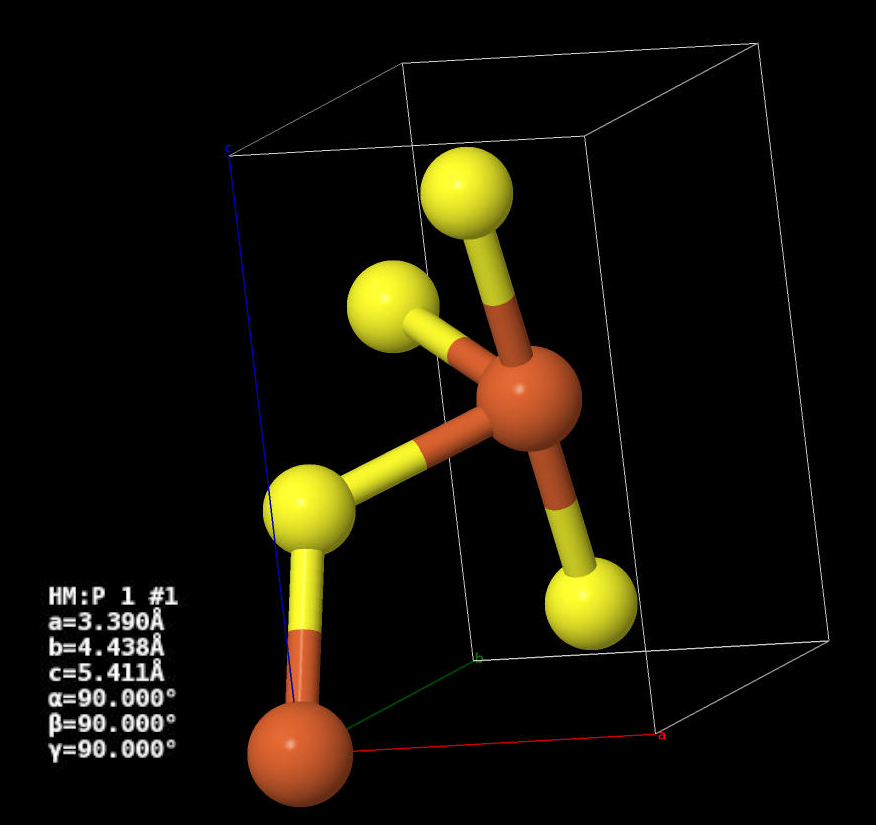
\includegraphics[width=0.61\textwidth]{images/primitiveCell}
\caption{Primitive cell of orthorhombic \ch{FeS2}.\\Materials Project (mp-1522), Jmol}
\label{fig:primitiveCell}
\end{figure}
\newpage
\section{Convergence studies and pseudopotentials}
In DFT computations, convergence studies are very important. They are meant to ensure that the chosen input parameters, like the cut-off energy (\texttt{ecut}) or the number of $k$-points in the cell (determined by the sampling of the Brillouin zone \texttt{ngkpt}), allow accurate results while limiting the computational time as much. To perform such an analysis, the same computations are repeated using datasets with various values of the parameter of interest, with an increasing accuracy of the environment. The evolution of some calculated variables, like the total energy of the unit cell (\texttt{etotal}), indicates when the parameters of interest guarantee a sufficiently accurate simulation.

In the following subsections, the convergence of the total energy per atom and of the lattice scale parameters will be studied with respect to \texttt{ecut} and \texttt{ngkpt}.
\subsection{Additional parameters}
To begin, we will use the \textit{Local Density Approximation} (LDA) functional. The pseudopotentials that will be used are retrieved from the PseudoDojo \cite{PseudoDojo}. Two pseudopotentials are used : the NC SR (ONCVPSP v0.4.1) LDA standard pseudopotential relative to Fe, and the same one but relative to S (both in psp8 format). The pseudopotentials respectively consider 16 electrons ($3s^23p^64s^23d^6$ for \ch{Fe}) and 6 electrons ($3s^23p^4$ for \ch{S}) so that the unit cell contains 56 electrons.

It is also important to properly define the parameters ruling the SCF procedure. The most important one is \texttt{nstep}, defining the number of allowed SCF cycles to reach convergence. It is set to \texttt{100} in the first place. \texttt{toldfe}, the difference of total energy between two SCF cycles defining the moment when convergence is reached, is set to \texttt{1.0d-10} Ha. \texttt{toldfe} is chosen as the structural relaxation is not performed yet (in that case, \texttt{toldff} or \texttt{tolrff} is preferably used). Although it is not mandatory, the SCF procedure can be preconditioned by specifying the macroscopic dielectric constant (\texttt{diemac}). It is used to speed up the SCF procedure. A value of \texttt{24} is chosen, accordingly to the Materials Project \cite{MaterialsProject}. 

Finally, the parameters of the $k$-points grid must be specified. \texttt{kptopt} is set to \texttt{1} in order to take advantage of the symmetry of the unit cell. 
By setting \texttt{prtkpt} to \texttt{1}, \texttt{Abinit} will generate a set of $k$-point grids, that will be helpful to optimize further computations and convergence studies.
\begin{center}
\begin{tabular}{lll}
\texttt{pseudos} & \multicolumn{2}{l}{\texttt{"pdj\_nc\_sr\_041\_lda\_standard\_psp8/Fe.psp8, pdj\_nc\_sr\_041\_lda\_standard\_psp8/S.psp8"}}\\
&&\\
\multicolumn{3}{l}{\texttt{\# parameters of the SCF procedure : }}\\
\texttt{nstep} & \texttt{100} &\texttt{\# maximal number of SCF cycles}\\
\texttt{toldfe} & \texttt{1.0d-10} &\texttt{\# SCF procedure will stop when the difference of total energy}\\
&&\texttt{\#\space\space\space\space between two iterations will be lower than toldfe Hartree}\\
\texttt{diemac} &\texttt{24.0} & \texttt{\# preconditioning of the SCF procedure.}\\
&&\\
\multicolumn{3}{l}{\texttt{\# parameters of the k-points grid : }}\\
\texttt{kptopt} & \texttt{1} &\\
\texttt{prtkpt} & \texttt{1} 
\end{tabular}
\end{center}
\subsection{Convergence of the total energy per atom as a function of the cut-off energy (\texttt{ecut})}
In the next computations, the default Monkhorst-Pack grids will be used. 4 $k$-points will be sampled along the longest lattice direction ([0 0 1]). To keep a constant density of $k$-points along each axis, 3 $k$-points will be sampled along directions [1 0 0] and  [0 1 0]. The input lattice parameters are thus :
\begin{center}
\begin{tabular}{lll}
\texttt{ngkpt} & \texttt{3 3 4}&\\
\texttt{nshiftk} & \texttt{1} &\\
\texttt{shiftk} &\texttt{0.5 0.5 0.5}
\end{tabular}
\end{center}
The study of the convergence of the simulation was performed by running \texttt{Abinit} with the input file \texttt{1522\_3\_ecutConv.abi} (\autoref{Abi1}).
The total energy per atom of the unit cell is then plotted versus \texttt{ecut} (which spans from $10$ [Ha] to $59$ [Ha]) (\autoref{fig:ecutConv}). Upper and lower bounds of $\pm 0.5$ [mHa] are set around the last obtained value. It allows to determine the first \texttt{ecut} for which the convergence is reasonable. In the present case, \texttt{ecut} = \texttt{40} [Ha].
\begin{figure}[H]
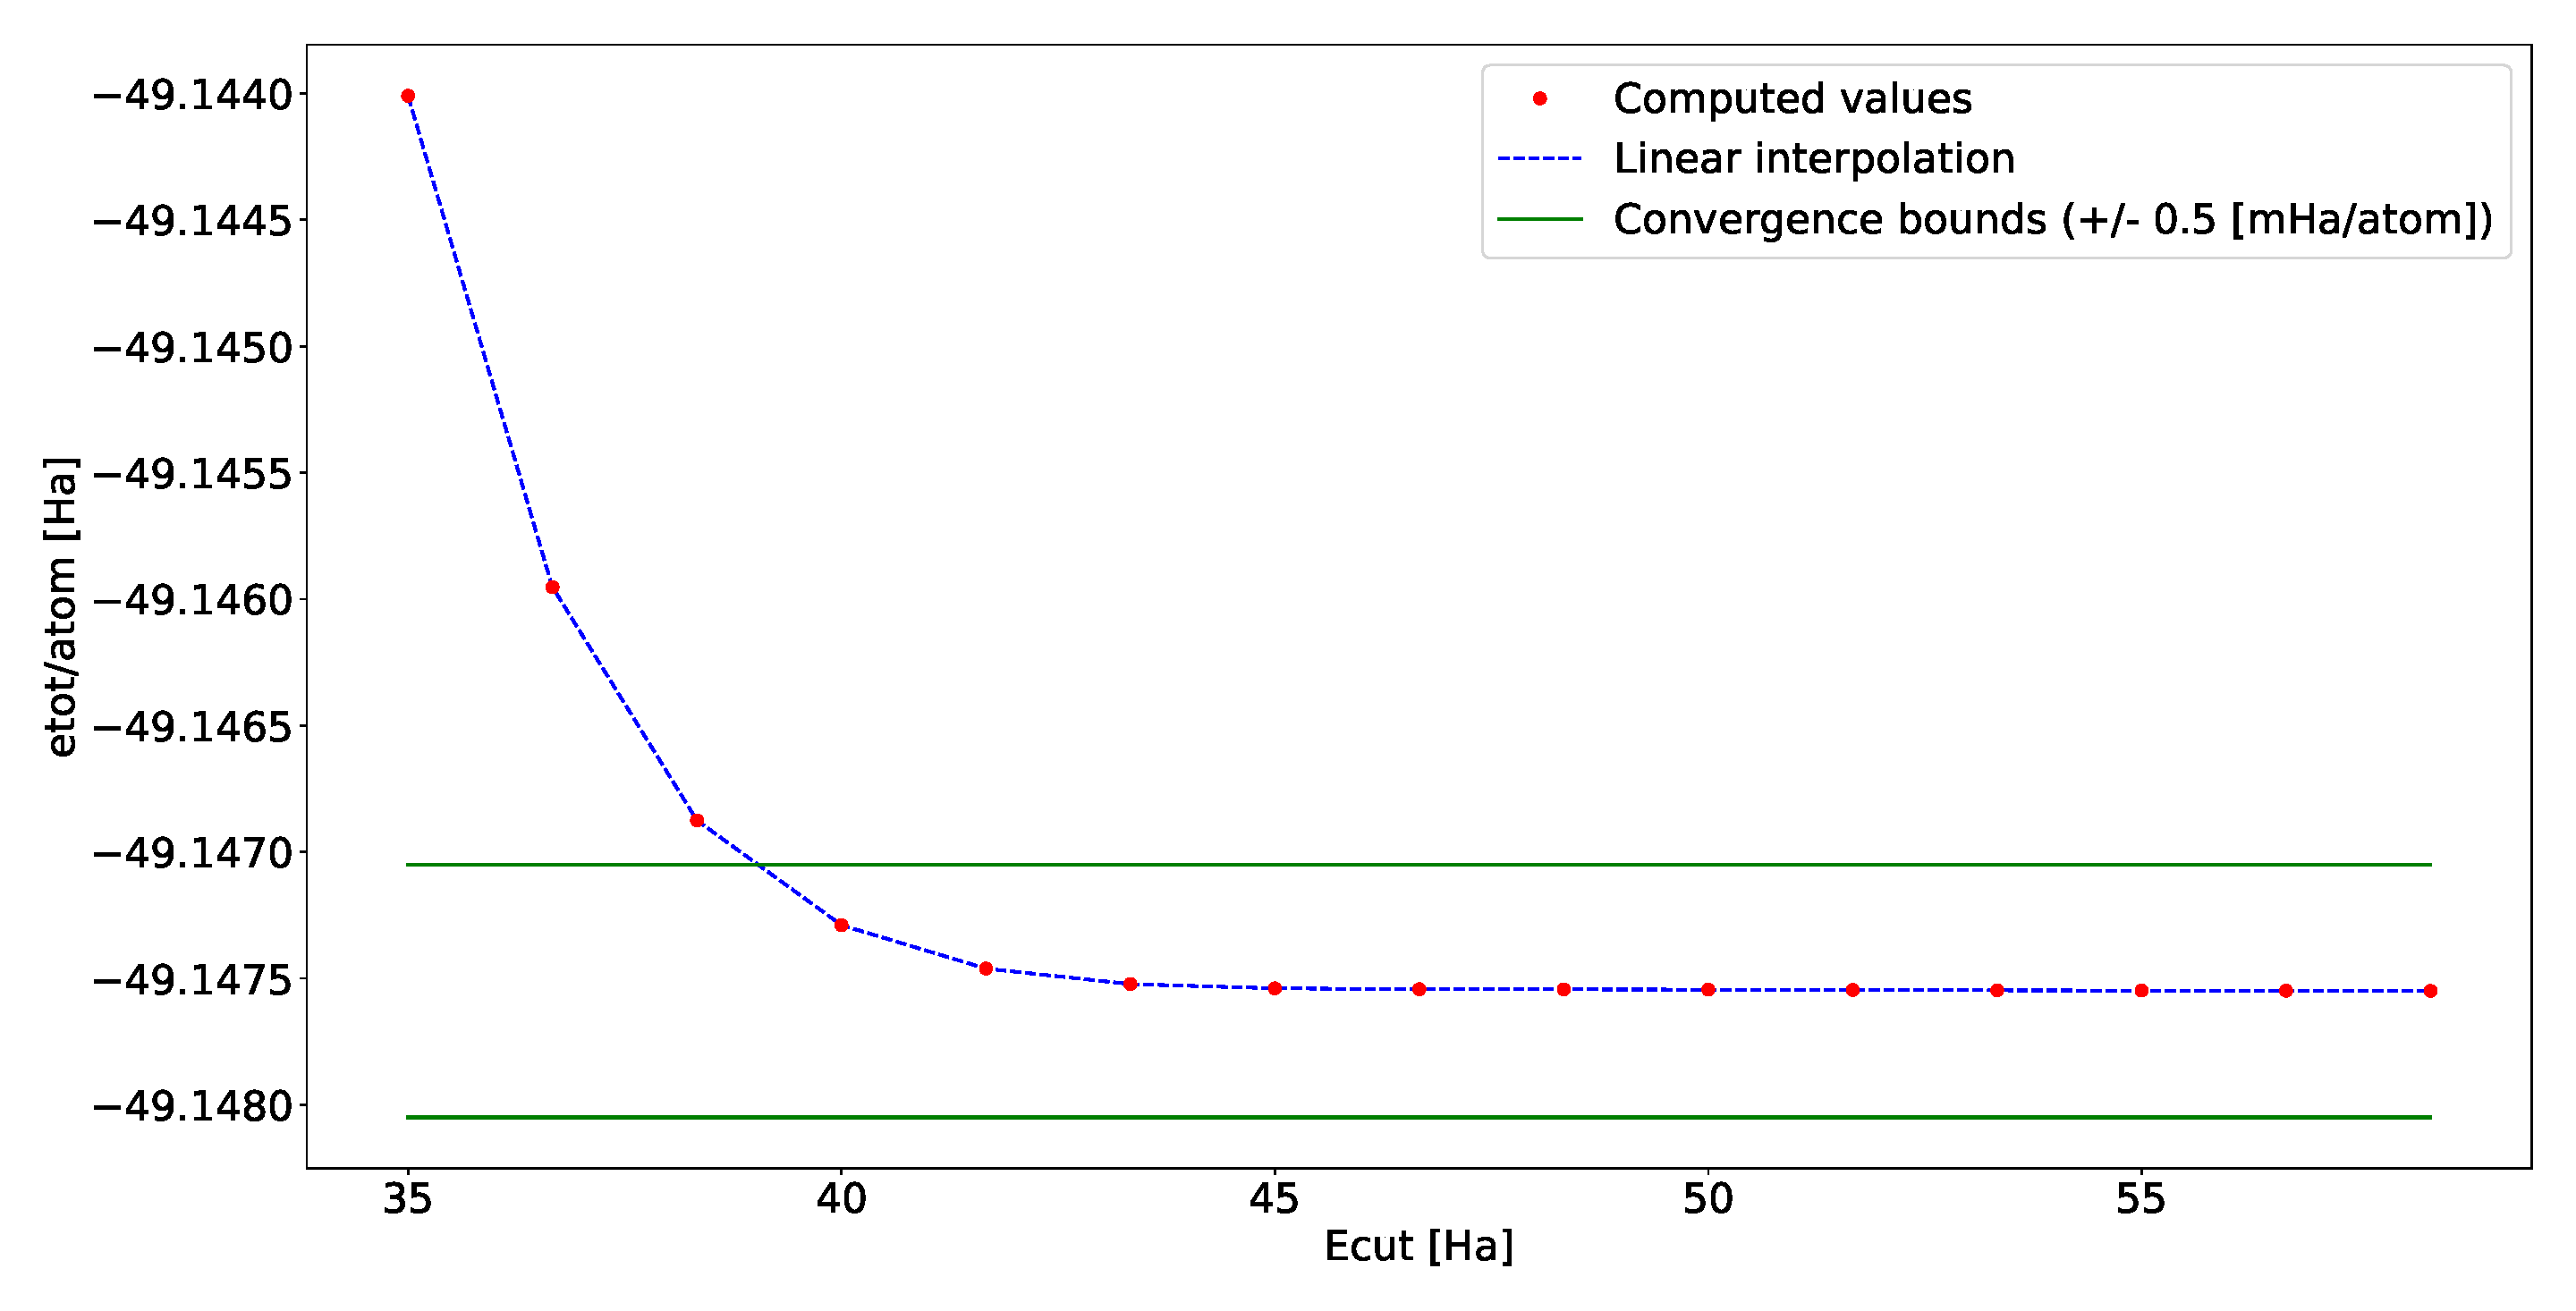
\includegraphics[width=\textwidth]{images/etotecut}
\caption{Total energy per atom as a function of the cut-off energy.\\
The \texttt{ecut} range is truncated for visual reasons.\\
Linear interpolations are shown as a guide for the eyes.}
\label{fig:ecutConv}
\end{figure}

\subsection{Convergence of the total energy per atom as a function of the number of $k$-points (\texttt{ngkpt})}
\label{convEtotNkpt}
Alternatively, the same kind of study is performed with respect to the number of $k$-points in the Brillouin zone. \texttt{Abinit} is run with the input file \texttt{1522\_4\_nkpConv.abi} (\autoref{Abi2}). The energy per atom can be plotted versus the \texttt{ngkpt} parameter (\autoref{fig:nkpConv}).
\begin{figure}[h]
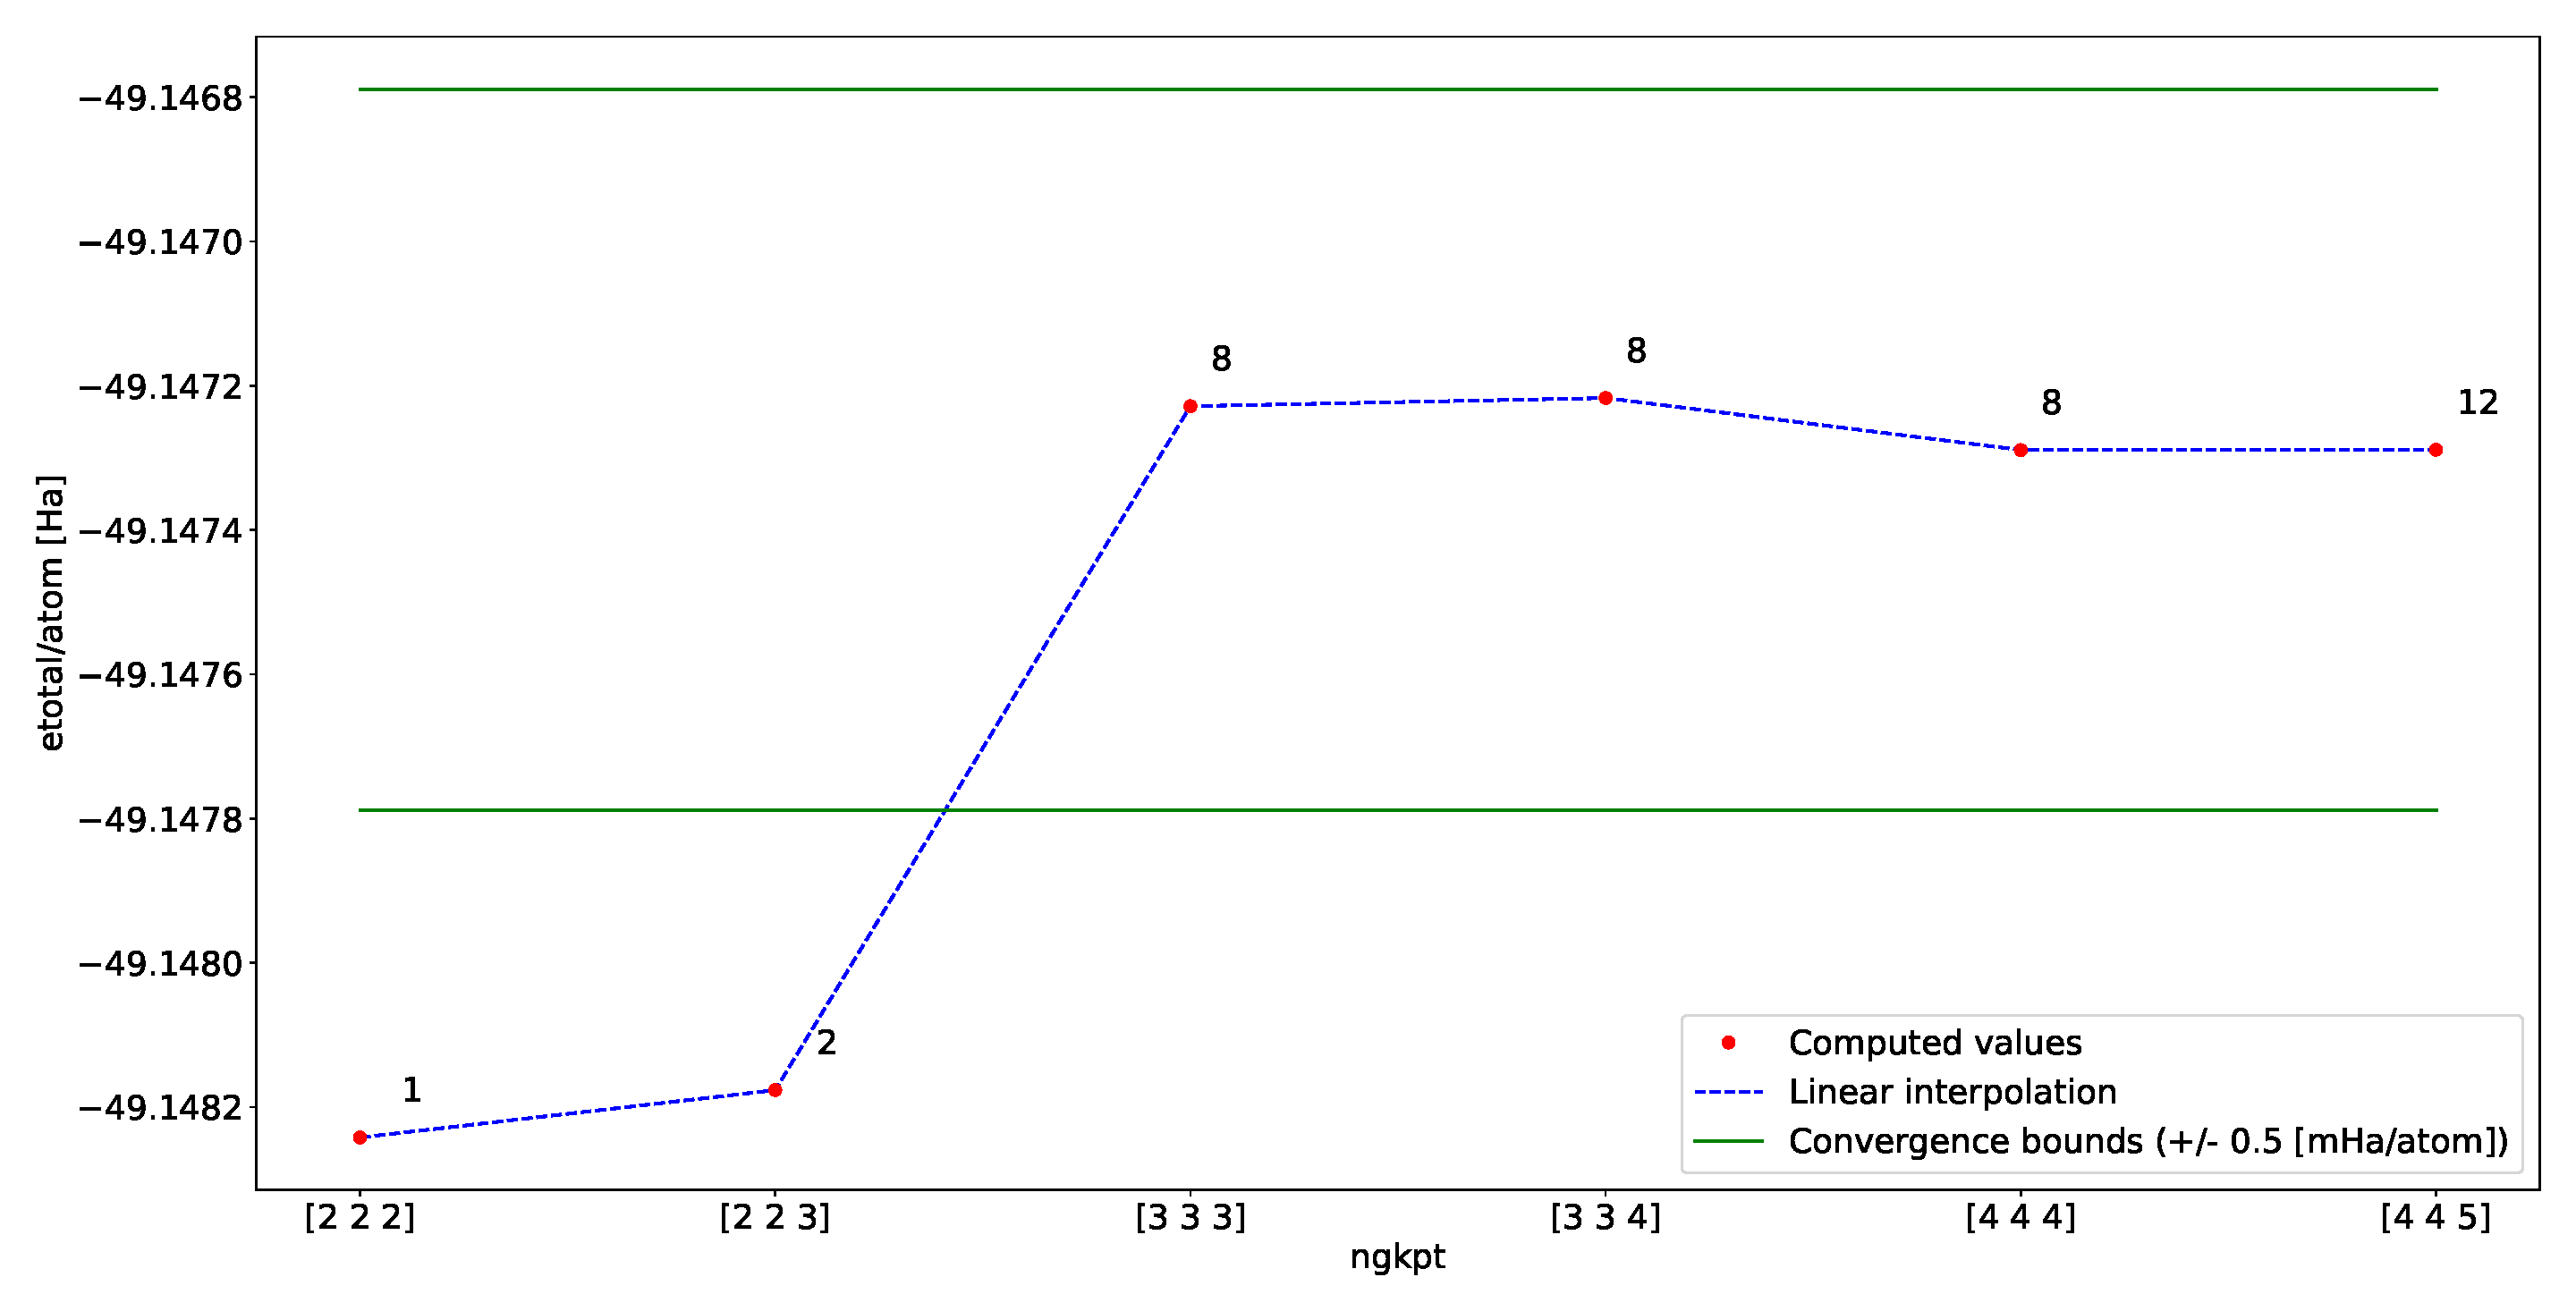
\includegraphics[width=\textwidth]{images/etotngkpt.pdf}
\caption{Total energy per atom as a function of the number of $k$-points in the $k$-points grid.\\
The number near each dot represents the corresponding number of $k$-points.
}
\label{fig:nkpConv}
\end{figure}
However, as the biggest and the smallest lattice scale parameters differs from 60\% in size, additional values of \texttt{ngkpt} keeping a similar $k$-sampling density along each axis are also tested.

The first converged \texttt{ngkpt} value is \texttt{[3 3 3]}.

Concerning the convergence of the total energy per atom, the couple of values (\texttt{ecut},\texttt{ngkpt}) that will be used in the further computations is thus (\texttt{40} [Ha],\texttt{[3 3 3]}).
\subsection{Convergence of \texttt{acell} as a function of the cut-off energy}
The convergence of the length scales of the unit cell was performed using a dataset of \texttt{ecut} values between $20$ [Ha] and $50$ [Ha], \texttt{ngkpt} = \texttt{[3 3 3]} and \texttt{ecutsm} = $0.5$ [Ha]. The input file used is \texttt{1522\_6\_acellEcutConv.abi} (\autoref{Abi3}). The results are displayed on \autoref{fig:acellecutconv}.
The first converged value is $30$ [Ha].
\begin{figure}
\centering
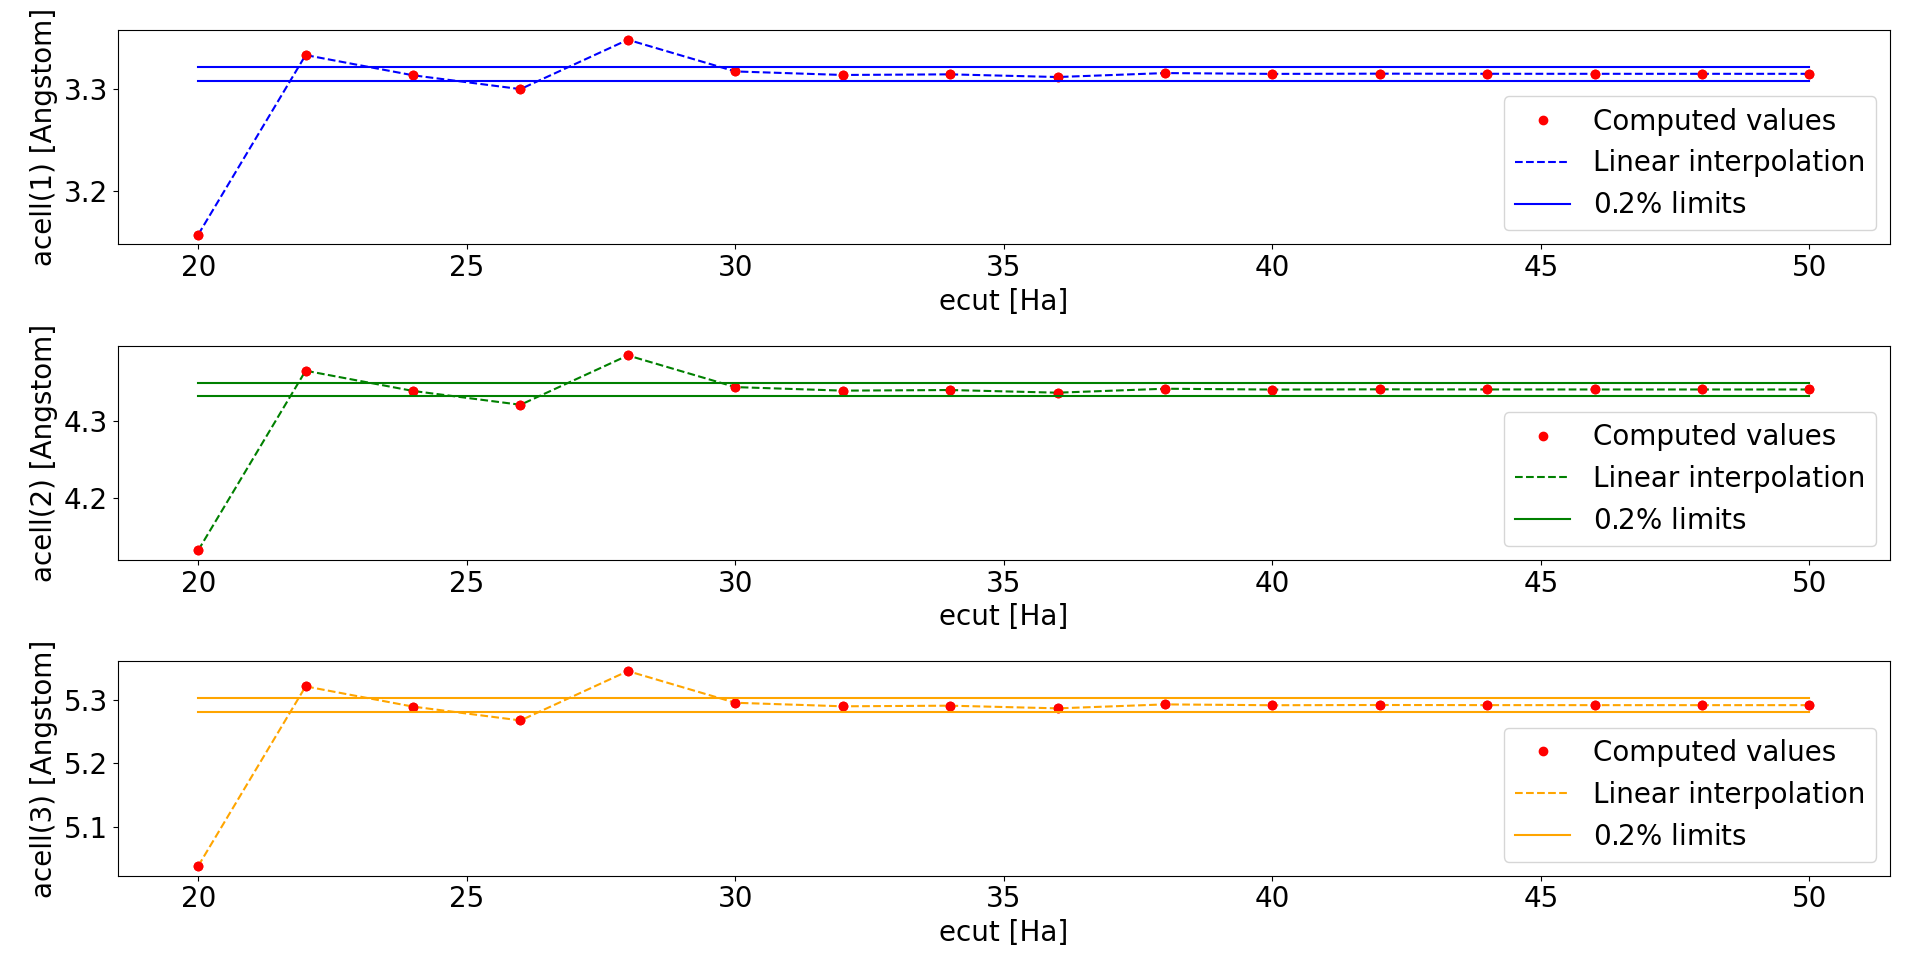
\includegraphics[width=\textwidth]{images/acellConv.png}
\caption{Convergence of the length scales \texttt{acell} as a function of the cut-off energy \texttt{ecut}.}
\label{fig:acellecutconv}
\end{figure}
\subsection{Convergence of \texttt{acell} as a function of the number of $k$-points}
The convergence of the length scales of the unit cell was analyzed with \texttt{ecut} = $40$ [Ha] and \texttt{ecutsm} = $0.5$ [Ha]. Additional values of \texttt{ngkpt} accounting for the conservation of a similar $k$-sampling density along the axis of the unit cell are also tested. The input file used is \texttt{1522\_3\_acellNgkptConv.abi} (\autoref{Abi4}). The results are displayed on \autoref{fig:acellnkpConv}. It can be seen that \texttt{[2 2 2]} is already in the limits of $0.2\%$ of the length. Therefore, the value \texttt{[2 2 2]} is considered as the first converged value.
\begin{figure}
\centering
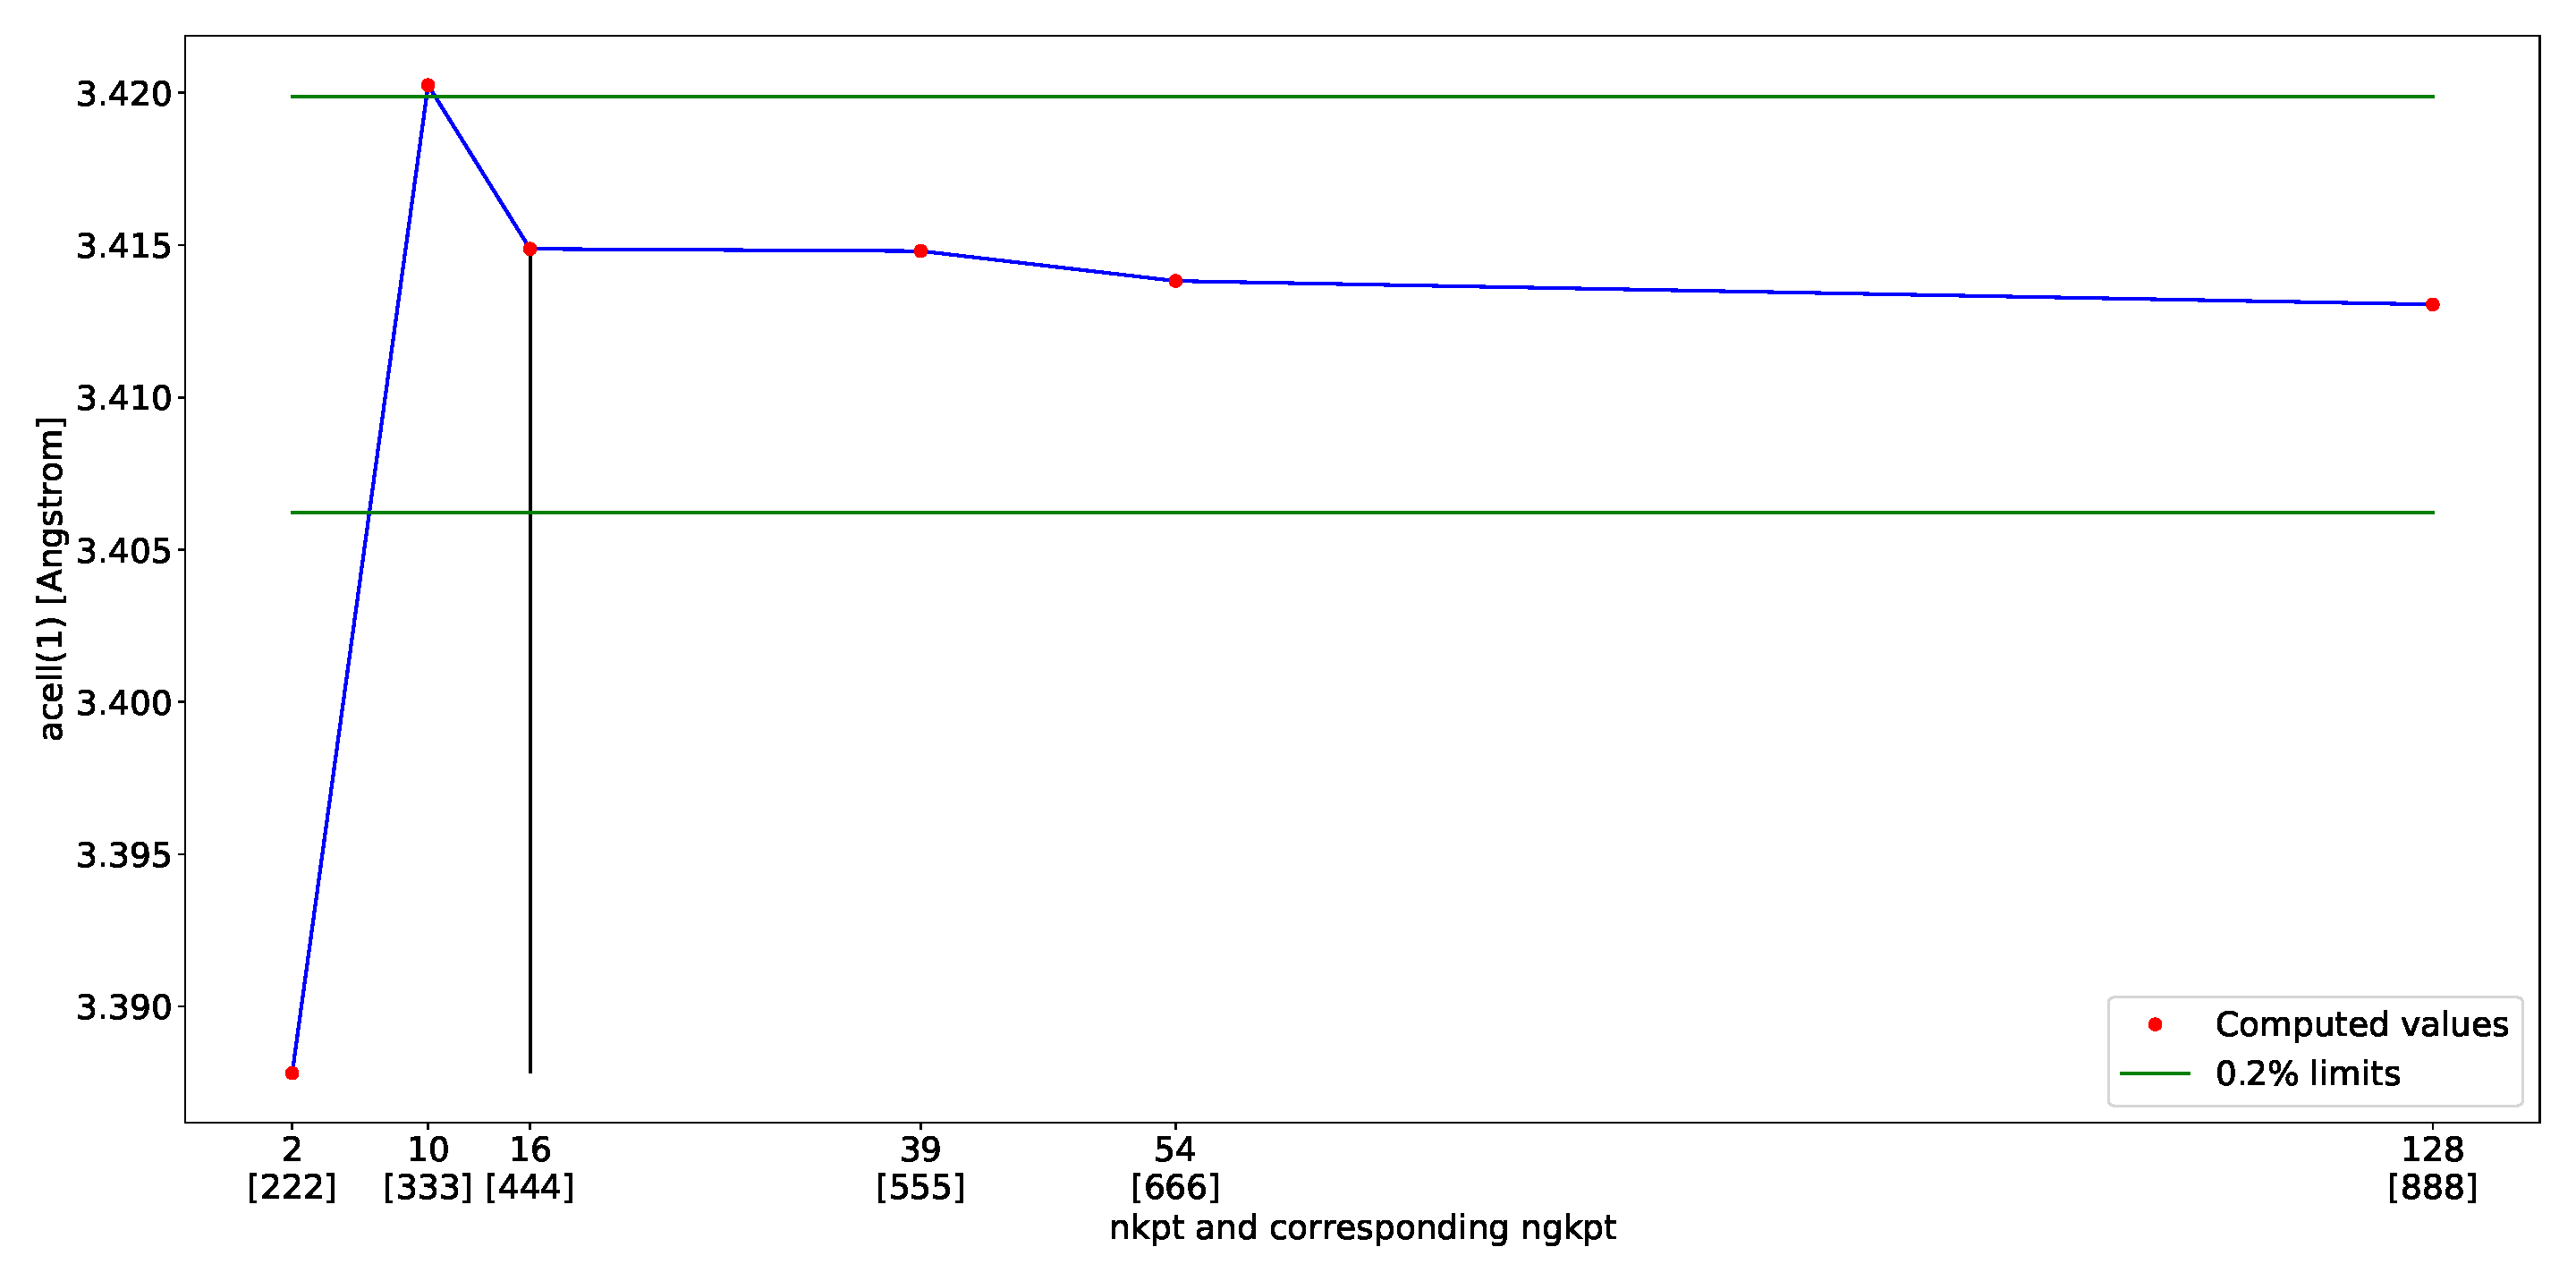
\includegraphics[width=\textwidth]{images/acellNgkpt.pdf}
\caption{Convergence of the length scales \texttt{acell} as a function of the number of $k$-points in the $k$-points grid.
The number near each dot represents the corresponding number of $k$-points.}
\label{fig:acellnkpConv}
\end{figure}
\subsection{Summary}
\begin{center}
\begin{tabular}{|l|c|c|}
\cline{2-3}   
\multicolumn{1}{c|}{}&\texttt{ecut [Ha]} & \texttt{ngkpt} \\
\hline
\multirow{1}{*}{Convergence of \texttt{etotal/atom}} & 40 & [3 3 3]\\
\hline
\multirow{1}{*}{Convergence of \texttt{acell}} & 30 & [2 2 2]\\   
\hline           
\end{tabular}
\end{center}
Furthermore, the most accurate value for \texttt{acell} and \texttt{xred}, obtained with \texttt{ngkpt} = \texttt{[4 4 5]} (\texttt{nkpt} = 12) and \texttt{ecut} = $40$ [Ha], is 
\begin{center}
\begin{tabular}{|c|c|}
\hline 
\texttt{acell(1)} & 6.2645 Bohr\\
\hline
\texttt{acell(2)} & 8.2011 Bohr\\
\hline
\texttt{acell(3)} & 9.9992 Bohr\\
\hline
\end{tabular}
\end{center}
or
\begin{center}
\begin{tabular}{|c|c|}
\hline
\texttt{acell(1)} & 3.315 Angstroms\\
\hline
\texttt{acell(2)} & 4.3398 Angstroms\\
\hline
\texttt{acell(3)} & 5.2913 Angstroms\\
\hline
\end{tabular}
\end{center}
and
\begin{center}
\begin{tabular}{|l|c|c|c|}
\cline{2-4}
\multicolumn{1}{l|}{}&\texttt{xred(1)} & \texttt{xred(2)} & \texttt{xred(3)}\\
\hline
\texttt{Fe \#1} & 0 & 0 & 0 \\
\hline
\texttt{Fe \#2} & 0.5 & 0.5 & 0.5\\
\hline
\texttt{S \#1} & 0 & 2.0809E-01 & 3.7374E-01\\
\hline
\texttt{S \#2} & 0& 7.9191E-01 & 6.2626E-01\\
\hline
\texttt{S \#3} & 0.5 & 2.9191E-01 & 8.7374E-01\\
\hline
\texttt{S \#4} & 0.5 & 7.0809E-01 & 1.2626E-01\\
\hline
\end{tabular}
\end{center}
\section{Optical properties}
\subsection{Electronic band structure}
The band structure of the material was computed as follows. First, an optimal $k$-path was obtained using \texttt{Abipy}. Then, 50 bands were analyzed using the parameters from the previous convergence studies (\texttt{ecut} = 30 Ha and \texttt{ngkpt} = [2 2 2]). A self-consistent density computation was done beforehand. The band structure is represented on \autoref{fig:bs}. From the data, the following values were obtained : 
\begin{center}
\begin{tabular}{|l|c|}
\hline
Fermi energy & $9.03565$ eV\\
\hline
Band gap & $0.735835$ eV\\
\hline
\end{tabular}
\end{center}
\begin{figure}[h]
\centering
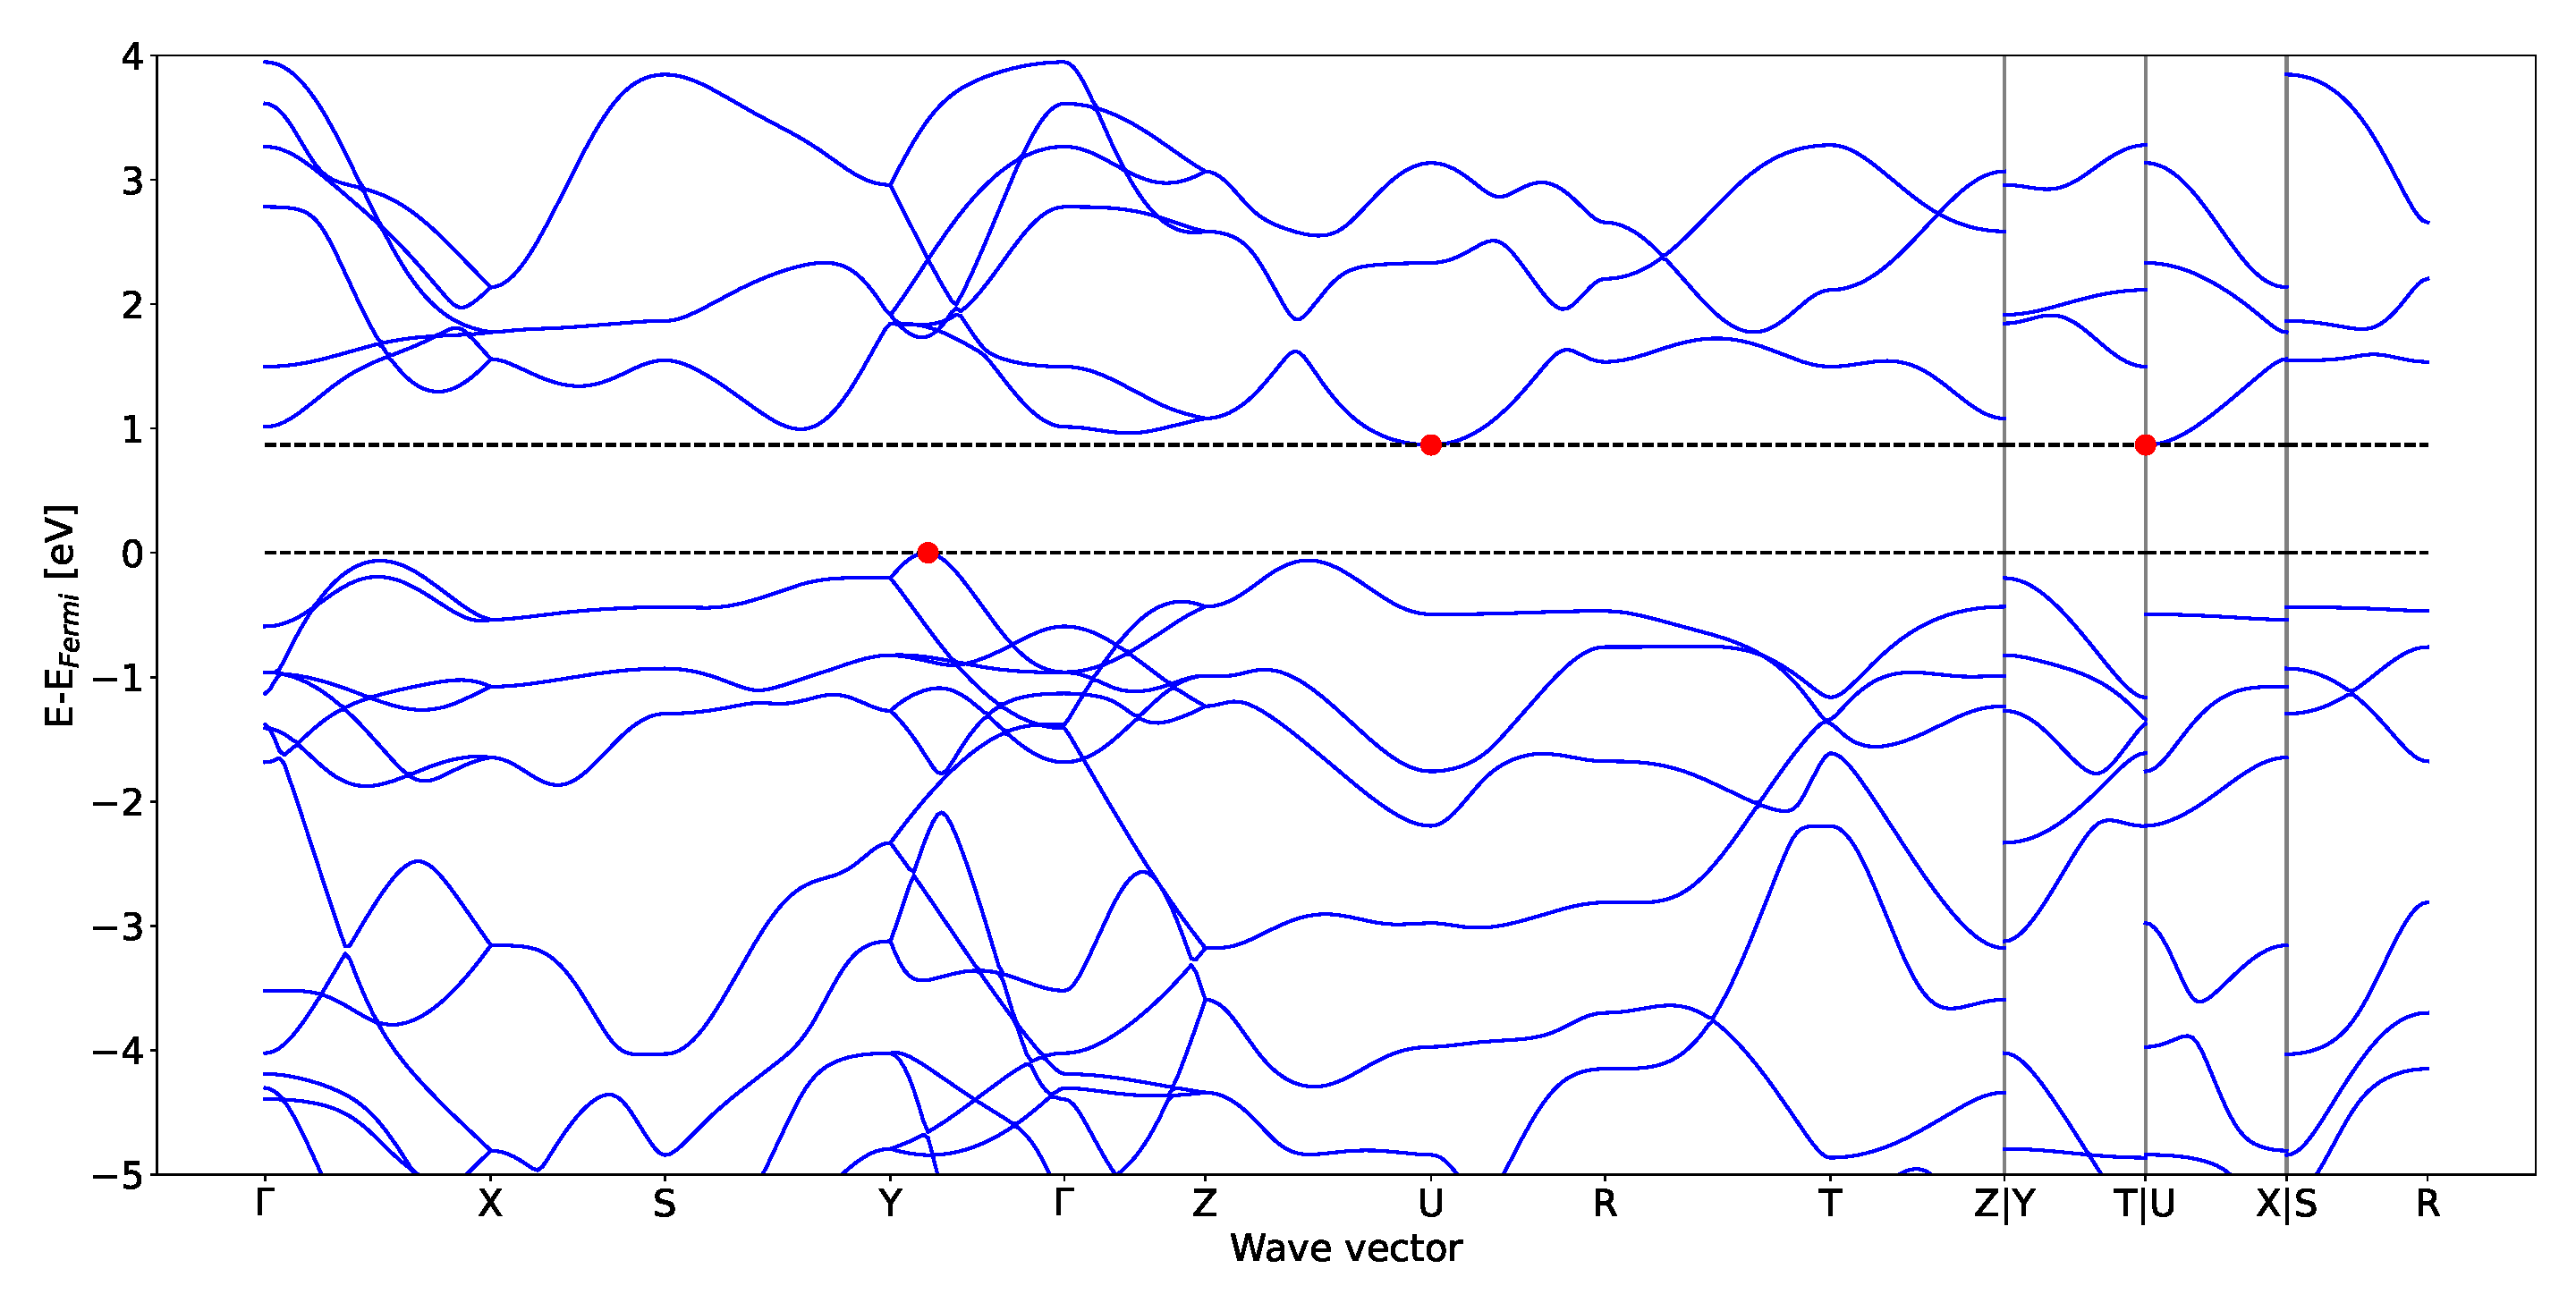
\includegraphics[width=\textwidth]{images/bs.pdf}
\caption{Band structure of \ch{FeS2}. The red dots represent the valence band minimums and the conduction band maximum.}
\label{fig:bs}
\end{figure}

\textcolor{blue}{
\textbackslash\textbackslash TODO\\
- Compute the electronic band structure\\
- compute the phonon dispersion\\
- Implications for a thin film used in a solar cell}
\newpage
\section{Comparison with the litterature}
\textcolor{blue}{
\textbackslash\textbackslash TODO\\
- Compare with the material project + other sources if needed\\
- Discuss the differences and the similitudes}
\newpage
\section{Conclusion}
\textcolor{blue}{
\textbackslash\textbackslash TODO\\
- Summary of the study
- What has been learned ? \\
- What implications in real life applications ?\\
- What further studies could be done ?}
\bibliographystyle{IEEEtran}
\bibliography{biblio}
\newpage
\appendix
\section{Convergence of the total energy per atom as a function of \texttt{ecut}}
\label{Abi1}
Name of the input file : \texttt{1522\_3\_ecutConv.abi}
\begin{center}
\begin{tabular}{lll}
\texttt{acell} & \texttt{3.390} \texttt{4.438} \texttt{5.411} \texttt{Angstr} & \\
\texttt{ntypat} & \texttt{2} &\\
\texttt{znucl} & \texttt{26 16}& \\
\texttt{natom} & \texttt{6} & \\
\texttt{typat} & \texttt{1 1 2 2 2 2}&\\
\texttt{xred} & \texttt{0\space\space\space\space\space\space 0\space\space\space\space\space\space 0} & \\
& \texttt{0.5\space\space\space\space 0.5\space\space\space\space0.5} & \\
& \texttt{0\space\space\space\space\space\space 0.206\space\space 0.3753} & \\
& \texttt{0\space\space\space\space\space\space 0.794\space\space 0.6247} & \\
& \texttt{0.5\space\space\space\space 0.294\space\space 0.8753} & \\
& \texttt{0.5\space\space\space\space 0.706\space\space 0.1247} & \\
&&\\
\texttt{pseudos} & \multicolumn{2}{l}{\texttt{"Fe.psp8,S.psp8"}}\\
&&\\
\multicolumn{3}{l}{\texttt{\# parameters of the SCF procedure : }}\\
\texttt{nstep} & \texttt{100} &\texttt{\# maximal number of SCF cycles}\\
\texttt{toldfe} & \texttt{1.0d-10} &\texttt{\# SCF procedure will stop when the difference of total}\\
&&\texttt{\#\space\space\space\space energy between two iterations will be lower than}\\
&&\texttt{\#\space\space\space\space toldfe Hartree}\\
\texttt{diemac} &\texttt{24.0} & \texttt{\# preconditioning of the SCF procedure.}\\
&&\\
\multicolumn{3}{l}{\texttt{\# parameters for generating the k-points grids : }}\\
\texttt{kptopt} & \texttt{1} &\\
\texttt{ngkpt} & \texttt{3 3 4}&\\
\texttt{nshiftk} &\texttt{1}&\\
\texttt{shiftk} &\texttt{0.5 0.5 0.5}&\\
&&\\
\texttt{ndtset} &\texttt{50}&\\
\texttt{ecut:}&\texttt{10}&\\
\texttt{ecut+}&\texttt{1}&\\ 
\end{tabular}
\end{center} 
\newpage
\section{Convergence of the total energy per atom as a function of \texttt{ngkpt}}
\label{Abi2}
Name of the input file : \texttt{1522\_4\_nkpConv.abi}
\begin{center}
\begin{tabular}{lll}
\texttt{acell} & \texttt{3.390} \texttt{4.438} \texttt{5.411} \texttt{Angstr} & \\
\texttt{ntypat} & \texttt{2} &\\
\texttt{znucl} & \texttt{26 16}& \\
\texttt{natom} & \texttt{6} & \\
\texttt{typat} & \texttt{1 1 2 2 2 2}&\\
\texttt{xred} & \texttt{0\space\space\space\space\space\space 0\space\space\space\space\space\space 0} & \\
& \texttt{0.5\space\space\space\space 0.5\space\space\space\space0.5} & \\
& \texttt{0\space\space\space\space\space\space 0.206\space\space 0.3753} & \\
& \texttt{0\space\space\space\space\space\space 0.794\space\space 0.6247} & \\
& \texttt{0.5\space\space\space\space 0.294\space\space 0.8753} & \\
& \texttt{0.5\space\space\space\space 0.706\space\space 0.1247} & \\
\texttt{ecut} &\texttt{40}&\texttt{\# the converged value for ecut} \\
&&\\
\texttt{pseudos} & \multicolumn{2}{l}{\texttt{"/Fe.psp8,S.psp8"}}\\
&&\\
\multicolumn{3}{l}{\texttt{\# parameters of the SCF procedure : }}\\
\texttt{nstep} & \texttt{100} &\texttt{\# maximal number of SCF cycles}\\
\texttt{toldfe} & \texttt{1.0d-10} &\texttt{\# SCF procedure will stop when the difference of total}\\
&&\texttt{\#\space\space\space\space energy between two iterations will be lower than}\\
&&\texttt{\#\space\space\space\space toldfe Hartree}\\
\texttt{diemac} &\texttt{24.0} & \texttt{\# preconditioning of the SCF procedure.}\\
&&\\
\multicolumn{3}{l}{\texttt{\# parameters for generating the k-points grids : }}\\
\texttt{getwfk} & \texttt{-1}&\\
\texttt{kptopt} & \texttt{1} &\\
\texttt{ndtset} & \texttt{6}&\\
\texttt{ngkpt1} & \texttt{2 2 2}&\\
\texttt{ngkpt2} & \texttt{2 2 3}&\\
\texttt{ngkpt3} & \texttt{3 3 3}&\\
\texttt{ngkpt4} & \texttt{3 3 4}&\\
\texttt{ngkpt5} & \texttt{4 4 4}&\\
\texttt{ngkpt6} & \texttt{4 4 5}&\\
\texttt{nshiftk} &\texttt{1}&\\
\texttt{shiftk} &\texttt{0.5 0.5 0.5}&
\end{tabular}
\end{center} 
\newpage
\section{Convergence of the lattice scale parameters as a function of \texttt{ecut}}
\label{Abi3}
Name of the input file : \texttt{1522\_6\_acellEcutConv.abi}
\begin{center}
\begin{tabular}{lll}
\texttt{acell} & \texttt{3.390} \texttt{4.438} \texttt{5.411} \texttt{Angstr} & \\
\texttt{ntypat} & \texttt{2} &\\
\texttt{znucl} & \texttt{26 16}& \\
\texttt{natom} & \texttt{6} & \\
\texttt{typat} & \texttt{1 1 2 2 2 2}&\\
\texttt{xred} & \texttt{0\space\space\space\space\space\space 0\space\space\space\space\space\space 0} & \\
& \texttt{0.5\space\space\space\space 0.5\space\space\space\space0.5} & \\
& \texttt{0\space\space\space\space\space\space 0.206\space\space 0.3753} & \\
& \texttt{0\space\space\space\space\space\space 0.794\space\space 0.6247} & \\
& \texttt{0.5\space\space\space\space 0.294\space\space 0.8753} & \\
& \texttt{0.5\space\space\space\space 0.706\space\space 0.1247} & \\
&&\\
\texttt{ndtset} &\texttt{16}&\\
\texttt{ecut:} &\texttt{20}&\\
\texttt{ecut+} &\texttt{2}&\\
&&\\
\texttt{pseudos} & \multicolumn{2}{l}{\texttt{"/Fe.psp8,S.psp8"}}\\
&&\\
\multicolumn{3}{l}{\texttt{\# parameters of the SCF procedure : }}\\
\texttt{nstep} & \texttt{100} &\texttt{\# maximal number of SCF cycles}\\
\texttt{toldff} & \texttt{1.0d-6} &\texttt{\# SCF procedure will stop when the difference of total}\\
&&\texttt{\#\space\space\space\space energy between two iterations will be lower than}\\
&&\texttt{\#\space\space\space\space toldfe Hartree}\\
\texttt{diemac} &\texttt{24.0} & \texttt{\# preconditioning of the SCF procedure.}\\
&&\\
\texttt{ionmov} & \texttt{2} &\\
\texttt{optcell} &\texttt{1}&\\
\texttt{dilatmx} &\texttt{1.05}&\\
\texttt{ecutsm} &\texttt{0.5}&\\
\texttt{kptopt}&\texttt{1}&\\
\texttt{ngkpt}&\texttt{3 3 3}&\\
\texttt{nshiftk}&\texttt{1}&\\
\texttt{shiftk}&\texttt{0.5 0.5 0.5}&\\
\texttt{getwfk}&\texttt{-1}&\\
\end{tabular}
\end{center} 
\newpage
\section{Convergence of the lattice scale parameters as a function of \texttt{ngkpt}}
\label{Abi4}
Name of the input file : \texttt{1522\_3\_acellNgkptConv.abi}
\begin{center}
\begin{tabular}{lll}
\texttt{acell} & \texttt{3.390} \texttt{4.438} \texttt{5.411} \texttt{Angstr} & \\
\texttt{ntypat} & \texttt{2} &\\
\texttt{znucl} & \texttt{26 16}& \\
\texttt{natom} & \texttt{6} & \\
\texttt{typat} & \texttt{1 1 2 2 2 2}&\\
\texttt{xred} & \texttt{0\space\space\space\space\space\space 0\space\space\space\space\space\space 0} & \\
& \texttt{0.5\space\space\space\space 0.5\space\space\space\space0.5} & \\
& \texttt{0\space\space\space\space\space\space 0.206\space\space 0.3753} & \\
& \texttt{0\space\space\space\space\space\space 0.794\space\space 0.6247} & \\
& \texttt{0.5\space\space\space\space 0.294\space\space 0.8753} & \\
& \texttt{0.5\space\space\space\space 0.706\space\space 0.1247} & \\
&&\\
\texttt{ndtset} &\texttt{6}&\\
\texttt{ngkpt1} &\texttt{2 2 2}&\\
\texttt{ngkpt2} &\texttt{2 2 3}&\\
\texttt{ngkpt3} &\texttt{3 3 3}&\\
\texttt{ngkpt4} &\texttt{3 3 4}&\\
\texttt{ngkpt5} &\texttt{4 4 4}&\\
\texttt{ngkpt6} &\texttt{4 4 5}&\\
&&\\
\texttt{ecut} &\texttt{40}&\\
\texttt{pseudos} & \multicolumn{2}{l}{\texttt{"/Fe.psp8,S.psp8"}}\\
&&\\
\multicolumn{3}{l}{\texttt{\# parameters of the SCF procedure : }}\\
\texttt{nstep} & \texttt{100} &\texttt{\# maximal number of SCF cycles}\\
\texttt{toldff} & \texttt{1.0d-6} &\texttt{\# SCF procedure will stop when the difference of total}\\
&&\texttt{\#\space\space\space\space energy between two iterations will be lower than}\\
&&\texttt{\#\space\space\space\space toldfe Hartree}\\
\texttt{diemac} &\texttt{24.0} & \texttt{\# preconditioning of the SCF procedure.}\\
&&\\
\texttt{ionmov} & \texttt{2} &\\
\texttt{optcell} &\texttt{1}&\\
\texttt{dilatmx} &\texttt{1.05}&\\
\texttt{ecutsm} &\texttt{0.5}&\\
\texttt{nshiftk}&\texttt{1}&\\
\texttt{shiftk}&\texttt{0.5 0.5 0.5}&\\
\texttt{getwfk}&\texttt{-1}&\\
\end{tabular}
\end{center} 
\end{document}